\documentclass[11pt,]{article}
\usepackage[left=1in,top=1in,right=1in,bottom=1in]{geometry}
\newcommand*{\authorfont}{\fontfamily{phv}\selectfont}
\usepackage[]{mathpazo}


  \usepackage[T1]{fontenc}
  \usepackage[utf8]{inputenc}



\usepackage{abstract}
\renewcommand{\abstractname}{}    % clear the title
\renewcommand{\absnamepos}{empty} % originally center

\renewenvironment{abstract}
 {{%
    \setlength{\leftmargin}{0mm}
    \setlength{\rightmargin}{\leftmargin}%
  }%
  \relax}
 {\endlist}

\makeatletter
\def\@maketitle{%
  \newpage
%  \null
%  \vskip 2em%
%  \begin{center}%
  \let \footnote \thanks
    {\fontsize{18}{20}\selectfont\raggedright  \setlength{\parindent}{0pt} \@title \par}%
}
%\fi
\makeatother




\setcounter{secnumdepth}{0}

\usepackage{color}
\usepackage{fancyvrb}
\newcommand{\VerbBar}{|}
\newcommand{\VERB}{\Verb[commandchars=\\\{\}]}
\DefineVerbatimEnvironment{Highlighting}{Verbatim}{commandchars=\\\{\}}
% Add ',fontsize=\small' for more characters per line
\usepackage{framed}
\definecolor{shadecolor}{RGB}{248,248,248}
\newenvironment{Shaded}{\begin{snugshade}}{\end{snugshade}}
\newcommand{\KeywordTok}[1]{\textcolor[rgb]{0.13,0.29,0.53}{\textbf{#1}}}
\newcommand{\DataTypeTok}[1]{\textcolor[rgb]{0.13,0.29,0.53}{#1}}
\newcommand{\DecValTok}[1]{\textcolor[rgb]{0.00,0.00,0.81}{#1}}
\newcommand{\BaseNTok}[1]{\textcolor[rgb]{0.00,0.00,0.81}{#1}}
\newcommand{\FloatTok}[1]{\textcolor[rgb]{0.00,0.00,0.81}{#1}}
\newcommand{\ConstantTok}[1]{\textcolor[rgb]{0.00,0.00,0.00}{#1}}
\newcommand{\CharTok}[1]{\textcolor[rgb]{0.31,0.60,0.02}{#1}}
\newcommand{\SpecialCharTok}[1]{\textcolor[rgb]{0.00,0.00,0.00}{#1}}
\newcommand{\StringTok}[1]{\textcolor[rgb]{0.31,0.60,0.02}{#1}}
\newcommand{\VerbatimStringTok}[1]{\textcolor[rgb]{0.31,0.60,0.02}{#1}}
\newcommand{\SpecialStringTok}[1]{\textcolor[rgb]{0.31,0.60,0.02}{#1}}
\newcommand{\ImportTok}[1]{#1}
\newcommand{\CommentTok}[1]{\textcolor[rgb]{0.56,0.35,0.01}{\textit{#1}}}
\newcommand{\DocumentationTok}[1]{\textcolor[rgb]{0.56,0.35,0.01}{\textbf{\textit{#1}}}}
\newcommand{\AnnotationTok}[1]{\textcolor[rgb]{0.56,0.35,0.01}{\textbf{\textit{#1}}}}
\newcommand{\CommentVarTok}[1]{\textcolor[rgb]{0.56,0.35,0.01}{\textbf{\textit{#1}}}}
\newcommand{\OtherTok}[1]{\textcolor[rgb]{0.56,0.35,0.01}{#1}}
\newcommand{\FunctionTok}[1]{\textcolor[rgb]{0.00,0.00,0.00}{#1}}
\newcommand{\VariableTok}[1]{\textcolor[rgb]{0.00,0.00,0.00}{#1}}
\newcommand{\ControlFlowTok}[1]{\textcolor[rgb]{0.13,0.29,0.53}{\textbf{#1}}}
\newcommand{\OperatorTok}[1]{\textcolor[rgb]{0.81,0.36,0.00}{\textbf{#1}}}
\newcommand{\BuiltInTok}[1]{#1}
\newcommand{\ExtensionTok}[1]{#1}
\newcommand{\PreprocessorTok}[1]{\textcolor[rgb]{0.56,0.35,0.01}{\textit{#1}}}
\newcommand{\AttributeTok}[1]{\textcolor[rgb]{0.77,0.63,0.00}{#1}}
\newcommand{\RegionMarkerTok}[1]{#1}
\newcommand{\InformationTok}[1]{\textcolor[rgb]{0.56,0.35,0.01}{\textbf{\textit{#1}}}}
\newcommand{\WarningTok}[1]{\textcolor[rgb]{0.56,0.35,0.01}{\textbf{\textit{#1}}}}
\newcommand{\AlertTok}[1]{\textcolor[rgb]{0.94,0.16,0.16}{#1}}
\newcommand{\ErrorTok}[1]{\textcolor[rgb]{0.64,0.00,0.00}{\textbf{#1}}}
\newcommand{\NormalTok}[1]{#1}

\usepackage{graphicx}
% We will generate all images so they have a width \maxwidth. This means
% that they will get their normal width if they fit onto the page, but
% are scaled down if they would overflow the margins.
\makeatletter
\def\maxwidth{\ifdim\Gin@nat@width>\linewidth\linewidth
\else\Gin@nat@width\fi}
\makeatother
\let\Oldincludegraphics\includegraphics
\renewcommand{\includegraphics}[1]{\Oldincludegraphics[width=\maxwidth]{#1}}

\title{Global Effects Of The Mexico City Policy  }



\author{\Large Joshua Keating, Peter Freschi, and John Harrison\vspace{0.05in} \newline\normalsize\emph{University of Washington}  }


\date{}

\usepackage{titlesec}

\titleformat*{\section}{\normalsize\bfseries}
\titleformat*{\subsection}{\normalsize\itshape}
\titleformat*{\subsubsection}{\normalsize\itshape}
\titleformat*{\paragraph}{\normalsize\itshape}
\titleformat*{\subparagraph}{\normalsize\itshape}


\usepackage{natbib}
\bibliographystyle{apsr}



\newtheorem{hypothesis}{Hypothesis}
\usepackage{setspace}

\makeatletter
\@ifpackageloaded{hyperref}{}{%
\ifxetex
  \usepackage[setpagesize=false, % page size defined by xetex
              unicode=false, % unicode breaks when used with xetex
              xetex]{hyperref}
\else
  \usepackage[unicode=true]{hyperref}
\fi
}
\@ifpackageloaded{color}{
    \PassOptionsToPackage{usenames,dvipsnames}{color}
}{%
    \usepackage[usenames,dvipsnames]{color}
}
\makeatother
\hypersetup{breaklinks=true,
            bookmarks=true,
            pdfauthor={Joshua Keating, Peter Freschi, and John Harrison (University of Washington)},
             pdfkeywords = {Mexico City policy, Global Gag Rule},  
            pdftitle={Global Effects Of The Mexico City Policy},
            colorlinks=true,
            citecolor=blue,
            urlcolor=blue,
            linkcolor=magenta,
            pdfborder={0 0 0}}
\urlstyle{same}  % don't use monospace font for urls



\begin{document}
	
% \pagenumbering{arabic}% resets `page` counter to 1 
%
% \maketitle

{% \usefont{T1}{pnc}{m}{n}
\setlength{\parindent}{0pt}
\thispagestyle{plain}
{\fontsize{18}{20}\selectfont\raggedright 
\maketitle  % title \par  

}

{
   \vskip 13.5pt\relax \normalsize\fontsize{11}{12} 
\textbf{\authorfont Joshua Keating, Peter Freschi, and John Harrison} \hskip 15pt \emph{\small University of Washington}   

}

}







\begin{abstract}

    \hbox{\vrule height .2pt width 39.14pc}

    \vskip 8.5pt % \small 

\noindent This document provides an introduction to R Markdown, argues for its
benefits, and presents a sample manuscript template intended for an
academic audience. I include basic syntax to R Markdown and a minimal
working example of how the analysis itself can be conducted within R
with the \texttt{knitr} package.


\vskip 8.5pt \noindent \emph{Keywords}: Mexico City policy, Global Gag Rule \par

    \hbox{\vrule height .2pt width 39.14pc}



\end{abstract}


\vskip 6.5pt

\noindent  \section{Introduction}\label{introduction}

The issue of abortion in the United States is one that is fiercely
debated and divides large segments of the population. These divides are
inherently partisan and therefore have led to legislation. In 1984 the
Reagan administration signed into law the ``Mexico City policy'', named
for the city in which it was signed. The policy requires all non
governmental organizations operating abroad to refrain from performing,
advising on or endorsing abortion as a method of family planning if they
wish to continue to receive receive federal funding. The policy has had
a tumultuous history, either being reinstated or rescinded depending on
the party affiliation of the current president. Starting with Bill
Clinton in 1993 the policy was rescinded, then restored by George W.
Bush in 2001, rescinded again by Barack Obama in 2009, and most recently
restored by Donald J. Trump in 2017.

At it's heart, the ban is propelled by the desire to limit the use of
U.S. taxpayer dollars to pay for abortion or abortion-related services.
The consequences of this ban include the termination of abortion related
services such as; education, family planning, counseling, and training.
The all or nothing nature of the ban would also cut off funds for non
abortion related health services that would be offered at non
governmental health providers. This presents some serious public health
concerns for areas of the world where these services are essential for
maternal health and prenatal care.

We hypothesized that the institution of the ban could lead to a
reduction in family planning services which could then lead to an
increase in induced abortions. By restricting the flow of funds into
health clinics that provide services related to abortion among others,
the U.S. government restricts the amount of care that can be provided to
those utilizing those services. The aim of this project was to gather,
analyze, and present data on the past effects of the Global Gag Rule and
create a resource that assists our audience in understanding the scope
of the policy, its observable impact on women's health, and the pathways
through which it influences public health policy decisions outside of
the United States.

\section{Related Work}\label{related-work}

At vero eos et accusamus et iusto odio dignissimos ducimus qui
blanditiis praesentium voluptatum deleniti atque corrupti quos dolores
et quas molestias excepturi sint occaecati cupiditate non provident,
similique sunt in culpa qui officia deserunt mollitia animi, id est
laborum et dolorum fuga. Et harum quidem rerum facilis est et expedita
distinctio. Nam libero tempore, cum soluta nobis est eligendi optio
cumque nihil impedit quo minus id quod maxime placeat facere possimus,
omnis voluptas assumenda est, omnis dolor repellendus. Temporibus autem
quibusdam et aut officiis debitis aut rerum necessitatibus saepe eveniet
ut et voluptates repudiandae sint et molestiae non recusandae. Itaque
earum rerum hic tenetur a sapiente delectus, ut aut reiciendis
voluptatibus maiores alias consequatur aut perferendis doloribus
asperiores repellat

This is an example of a footer\footnote{Testing custom footer} Here is
another example\footnote{testting second footer} This is useful for both
debugging and the publication stage, when the editorial team will ask
for the raw \texttt{.tex} so that they could render it and later provide
page proofs.

\section{Methods}\label{methods}

Heres some emmbeded code

\begin{Shaded}
\begin{Highlighting}[]
\CommentTok{# lmfit <- lm(Maternal_Mortality ~ Exposure + Num.Ab, data=full.exposure.mm,}
\CommentTok{# na.action = na.omit) lmfit preds <- predict(lmfit) plot(preds,}
\CommentTok{# full.exposure.mm$Maternal_Mortality[!is.na(full.exposure.mm$Num.Ab)])}

\NormalTok{tmp <-}\StringTok{ "test"}
\end{Highlighting}
\end{Shaded}

At vero eos et accusamus et iusto odio dignissimos ducimus qui
blanditiis praesentium voluptatum deleniti atque corrupti quos dolores
et quas molestias excepturi sint occaecati cupiditate non provident,
similique sunt in culpa qui officia deserunt mollitia animi, id est
laborum et dolorum fuga. Et harum quidem rerum facilis est et expedita
distinctio. Nam libero tempore, cum soluta nobis est eligendi optio
cumque nihil impedit quo minus id quod maxime placeat facere possimus,
omnis voluptas assumenda est, omnis dolor repellendus. Temporibus autem
quibusdam et aut officiis debitis aut rerum necessitatibus saepe eveniet
ut et voluptates repudiandae sint et molestiae non recusandae. Itaque
earum rerum hic tenetur a sapiente delectus, ut aut reiciendis
voluptatibus maiores alias consequatur aut perferendis doloribus
asperiores repellat

need to fix this spacing here

\begin{figure}
\centering
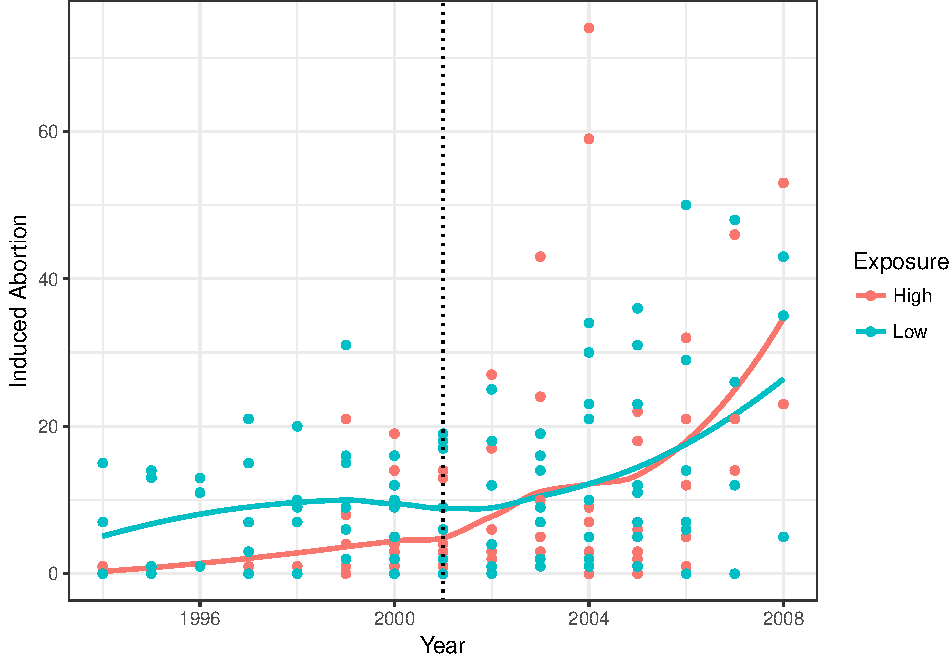
\includegraphics{final-paper_files/figure-latex/unnamed-chunk-2-1.pdf}
\caption{Abortion Rates For Both Levels Of Exposure}
\end{figure}

\section{Results}\label{results}

At vero eos et accusamus et iusto odio dignissimos ducimus qui
blanditiis praesentium voluptatum deleniti atque corrupti quos dolores
et quas molestias excepturi sint occaecati cupiditate non provident,
similique sunt in culpa qui officia deserunt mollitia animi, id est
laborum et dolorum fuga. Et harum quidem rerum facilis est et expedita
distinctio. Nam libero tempore, cum soluta nobis est eligendi optio
cumque nihil impedit quo minus id quod maxime placeat facere possimus,
omnis voluptas assumenda est, omnis dolor repellendus. Temporibus autem
quibusdam et aut officiis debitis aut rerum necessitatibus saepe eveniet
ut et voluptates repudiandae sint et molestiae non recusandae. Itaque
earum rerum hic tenetur a sapiente delectus, ut aut reiciendis
voluptatibus maiores alias consequatur aut perferendis doloribus
asperiores repellat

\section{Discussion}\label{discussion}

At vero eos et accusamus et iusto odio dignissimos ducimus qui
blanditiis praesentium voluptatum deleniti atque corrupti quos dolores
et quas molestias excepturi sint occaecati cupiditate non provident,
similique sunt in culpa qui officia deserunt mollitia animi, id est
laborum et dolorum fuga. Et harum quidem rerum facilis est et expedita
distinctio. Nam libero tempore, cum soluta nobis est eligendi optio
cumque nihil impedit quo minus id quod maxime placeat facere possimus,
omnis voluptas assumenda est, omnis dolor repellendus. Temporibus autem
quibusdam et aut officiis debitis aut rerum necessitatibus saepe eveniet
ut et voluptates repudiandae sint et molestiae non recusandae. Itaque
earum rerum hic tenetur a sapiente delectus, ut aut reiciendis
voluptatibus maiores alias consequatur aut perferendis doloribus
asperiores repellat

\begin{figure}
\centering
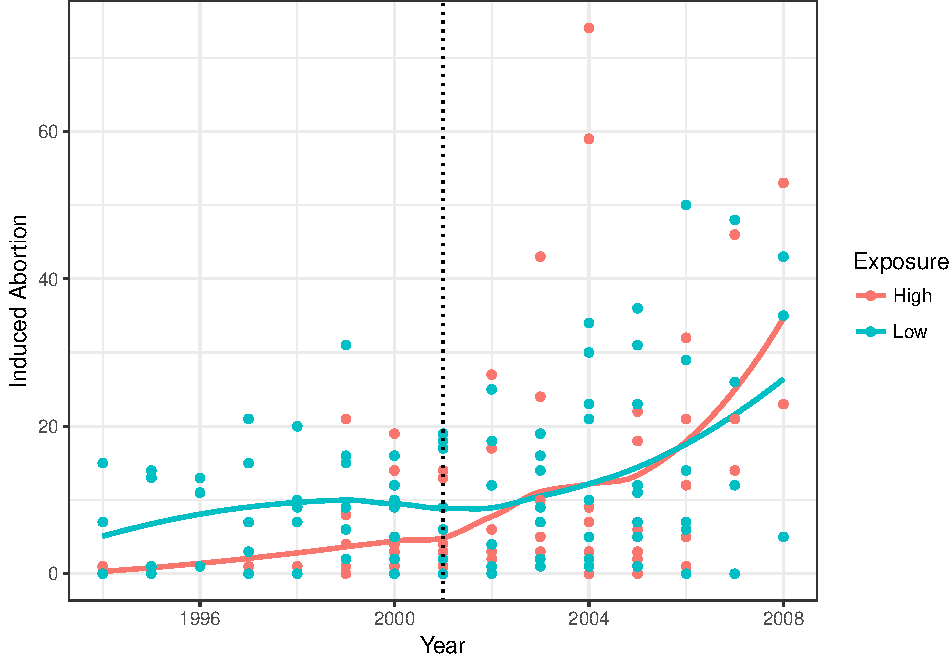
\includegraphics{final-paper_files/figure-latex/unnamed-chunk-3-1.pdf}
\caption{Test}
\end{figure}

\section{Future Work}\label{future-work}

At vero eos et accusamus et iusto odio dignissimos ducimus qui
blanditiis praesentium voluptatum deleniti atque corrupti quos dolores
et quas molestias excepturi sint occaecati cupiditate non provident,
similique sunt in culpa qui officia deserunt mollitia animi, id est
laborum et dolorum fuga. Et harum quidem rerum facilis est et expedita
distinctio. Nam libero tempore, cum soluta nobis est eligendi optio
cumque nihil impedit quo minus id quod maxime placeat facere possimus,
omnis voluptas assumenda est, omnis dolor repellendus. Temporibus autem
quibusdam et aut officiis debitis aut rerum necessitatibus saepe eveniet
ut et voluptates repudiandae sint et molestiae non recusandae. Itaque
earum rerum hic tenetur a sapiente delectus, ut aut reiciendis
voluptatibus maiores alias consequatur aut perferendis doloribus
asperiores repellat

\newpage
\singlespacing 
\end{document}
